% V3 Chinese native LaTeX manuscript. Compile with: xelatex main.tex
\documentclass[UTF8,10pt,a4paper,twocolumn]{ctexart}
\usepackage[margin=2.0cm]{geometry}
\usepackage{amsmath,amssymb,booktabs,longtable,array,graphicx,float}
\usepackage[numbers,sort&compress]{natbib}
\usepackage{hyperref,xurl}
\hypersetup{colorlinks=true,linkcolor=black,citecolor=blue,urlcolor=blue}
\setlength{\columnsep}{0.75cm}
\graphicspath{{../../v2/figs/}}
\title{证据约束的无标签中子电流时序诊断辅助}
\author{作者信息待补充}
\date{}
\begin{document}
\maketitle

\begin{abstract}
待在中文正文与图表稳定后撰写。
\end{abstract}

\noindent\textbf{关键词：}中子仪表；无标签时序；诊断辅助；可追溯观测；检索增强；证据溯源

\input{sections/01_introduction_zh}
\section{相关工作}

数据驱动的工业时序故障诊断已形成成熟路线，其通常以预先定义的诊断任务、可用标签或可控的故障场景为基础。这些前提使模型性能能够通过分类或识别指标进行比较，但也限制了方法直接迁移到缺乏统一故障真值的现场历史档案。

核工程数据方法的范围远不止中子信号分析。一类工作依托物理模型、状态重建和先进数值模拟服务于反应堆监测与安全研究；CORTEX、McSAFER 和 METIS 等项目体现了这一建模与验证路线 \citep{demaziere2022cortex}。另一类工作面向核电厂运行中的在线监测与仪表通道评估，已形成明确的工程和维护支持基础 \citep{iaea2008olm1,iaea2008olm2,hashemian2011online}。在信号层面，中子噪声研究为非侵入式分析反应堆运行和中子测量系统相关现象提供了方法基础；围绕中子探测器验证和核电厂故障诊断的数据驱动研究，也已在预设信号构造或故障场景下开展 \citep{pazsit2010noise,tambouratzis2020neutron,tambouratzis2020decomposition,elbordany2024fault}。

通用语言代理与工具调用研究表明，语言模型可以规划动作、调用外部工具，并将工具输出纳入后续推理，而不必直接承担全部专业计算 \citep{yao2023react,schick2023toolformer,patil2024gorilla}。专业诊断系统进一步展示了这种分工的具体形态：ChatCAD 将专用 CAD 网络的分类、分割和报告结果转换为文本表示后交由语言模型整合 \citep{wang2024chatcad}；AgentMD 则将临床计算器构建为可执行工具，并由语言代理选择和调用 \citep{jin2025agentmd}。这些研究共同说明，专业模型或确定性工具可以保留对底层测量和计算的职责，而语言模型承担跨工具的信息组织。

在核工程中，这种职责划分还需要满足来源可追溯、技术术语受控和工程师复核等要求。现有核领域语言模型研究已探索诊断可靠性、预测性维护中的技术语言生成、核电厂文档解释，以及面向安全关键决策支持的检索增强框架 \citep{reeves2024reliability,lin2025cws,mapes2025uprate,ndum2026radiant}。这些工作为核工程中语言模型的可靠使用提供了直接基础，但其主要输入仍是技术文档、维护语境或已有的文本问题，而非无标签的原始仪表时序。

检索增强生成通过外部资料为知识密集型生成提供依据 \citep{lewis2020rag}。除端到端回答质量外，近年来的 RAG 评价也开始区分检索模块与生成模块的失效模式；例如 RAGChecker 将评价细化到检索和生成的多个环节 \citep{ru2024ragchecker}。这一视角对于核工程尤其重要：预先指定的重要来源是否仍进入检索结果前列、段落能否定位以及陈述是否受到证据支持，不能被单一相似度分数或语言流畅性所替代。现有核工程技术文本研究已关注检索、事实性、来源追溯和人工验证 \citep{reeves2024reliability,lin2025cws,mapes2025uprate,ndum2026radiant}，为安全相关场景中的证据定位、引用和人工复核提供了重要基础。

总体而言，现有研究分别覆盖了工业时序诊断、专业工具调用和技术文档 RAG；对于无统一故障真值的核仪表历史档案，如何将可追溯的测量侧观察与受来源策略约束的证据侧解释衔接起来，仍构成本文关注的研究缺口。

\section{无标签中子电流档案的可追溯观测与证据约束解释}

本研究将两类性质不同的资源置于同一诊断辅助流程中：一类是核电厂运行环境中积累的中子电流历史记录，用于形成可复核的信号现象；另一类是核仪表与控制技术资料，用于提供可定位的文献证据。二者都不是故障标签库。前者不能仅凭波形确认设备故障，后者也不能脱离测量现象直接解释某段原始信号。本章据此明确研究对象、两侧任务及其受控连接方式。

\subsection{研究对象、数据结构与披露边界}

测量资源来自同一核电厂采集周期内的中子电流历史档案。档案包含 42 条多通道 CSV 记录，来自四套仪表组。每条记录由时间列和 7 个中子电流通道组成；典型记录约含 $6\times10^{5}$ 个样本，采样间隔约为 1 s，并覆盖多日窗口。组内通道具有相对布置关系，因此其顺序不是任意的特征排列。原始导出文件可能含有局部时间戳紊乱或非单调片段，时间顺序校正因而是后续分析的前提。

档案不随每段时序提供完整的运行工况、维护历史和故障确认记录。反应堆型号、厂站身份、具体仪表系统名称及其他可识别信息亦暂不公开；本章只保留理解数据组织、方法适用范围和结果解释所必需的信息。本文据此关注可被复核的时间变化、通道间关系和信号完整性线索，而不依据记录推断反应堆型号或直接重建反应堆物理状态。

\subsection{测量侧：从原始记录到 observation packet}

测量侧的产物不是故障分类结果，而是一份 \textbf{observation packet}：它说明对哪一条记录、以哪些确定性规则、观察到了哪些数据质量和信号现象。确定性脚本将结构化观测写入记事板；其中稳定字段直接形成供后续检索使用的 compact alert summary，测量侧 agent 则只读取这些已保存结果，组织面向工程师阅读的 condition report。二者均不构成对物理机理、设备状态或根因的确认。

\begin{figure*}[!t]
  \centering
  \begin{minipage}[t]{0.263\textwidth}
    \centering\textbf{(a)}\par\vspace{1mm}
    
\includegraphics[width=\linewidth]{fig03a_spike_rule_example}
  \end{minipage}\hfill
  \begin{minipage}[t]{0.341\textwidth}
    \centering\textbf{(b)}\par\vspace{1mm}
    
\includegraphics[width=\linewidth]{fig03b_pearson_example}
  \end{minipage}\hfill
  \begin{minipage}[t]{0.296\textwidth}
    \centering\textbf{(c)}\par\vspace{1mm}
    
\includegraphics[width=\linewidth]{fig03c_lag_example}
  \end{minipage}
  \caption{确定性 probes 所描述的统计现象示例：(a) 样本 2600--2720 的局部稳健偏离规则，纵轴为相应通道记录的中子电流值；(b) 通道间 Pearson 共变；(c) 相关--滞后扫描。它们用于说明 observation packet 中可保存的描述性证据，不构成已确认故障或因果方向。}
  \label{fig:probe-examples}
\end{figure*}

\subsubsection{初始化、数据健康与分析单元}

每次分析以一条记录为单位。初始化脚本解析时间列、按时间排序，并生成唯一的 active record；同时记录样本数、名义采样间隔、缺失情况和不活跃通道等数据健康信息。后续分析不再接受自由指定的原始文件路径，而是从该分析单元读取 active record。这样可以使一组观测始终对应同一输入记录，并保留输入、参数、脚本版本和派生产物之间的关联。

这一安排并不要求忽略数据结构或通道相对位置；相反，通道标识和组内相对关系是组织观察所必需的先验。其限制在于，测量侧不把这些结构信息延伸为预设故障知识，也不把任一统计量直接翻译为设备故障类别。

\subsubsection{预先定义的确定性分析工具}

初始化完成后，脚本仅执行预先注册的 probes，覆盖数据健康、形态与共变、事件与区段、同步与滞后、极值定位和截面快照等观察。各工具将输入范围、参数与结构化输出写入 observation packet；图~\ref{fig:probe-examples} 展示其中三类统计现象。形态和共变扫描提供的是信号关系的初步描述。例如，较高的两两相关性可以提示共享变化、可能的冗余或需要结合通道位置进一步核查的情形，但它本身不证明仪表关系或物理机制。相同地，相关—滞后扫描只区分近同步与时间错位的统计模式，不赋予因果方向。

为使事件识别可重复，当前实现对每个通道采用长度为 31 个样本的中心滑动窗口；记录边界处使用可获得的窗口样本。令 $W_t$ 为时刻 $t$ 的窗口，$x_{t,c}$ 为通道 $c$ 的电流值，则局部基线、点态绝对残差及其稳健局部尺度定义为

\[
\begin{aligned}
m_{t,c} &= \operatorname{median}_{\tau\in W_t}x_{\tau,c},\\
r_{t,c} &= \left|x_{t,c}-m_{t,c}\right|,\\
d_{t,c} &= \operatorname{median}_{\tau\in W_t}r_{\tau,c},\\
R_c &= \max_t x_{t,c}-\min_t x_{t,c}.
\end{aligned}
\]

这类以中位数和绝对偏差抑制局部异常影响的稳健估计思想，可追溯至相关基础研究 \citep{hampel1974influence,rousseeuw1993alternatives}。对于非恒定通道，突刺候选定义为同时满足局部与全程幅度条件的点：

\[
I^{\mathrm{spike}}_{t,c}=
\mathbb{I}\!\left(r_{t,c}>5d_{t,c}\right)
\mathbb{I}\!\left(r_{t,c}>0.05R_c\right).
\]

连续的阳性点合并为一个短时偏离事件；长度不超过两个采样点的连续零值段另行记录。该规则同时响应向上和向下的短时偏离，因而此处的“突刺”仅指检测事件，不预设其物理方向或故障含义。两通道之间以 Pearson 相关系数描述共变，当前实现将 $r\geq0.99$ 标记为近冗余，将 $0.85\leq r<0.99$ 标记为强共变。这些阈值是用于稳定生成 observation packet 的操作性规则，而非故障判据；参数敏感性说明可置于附录或补充材料。

\subsubsection{报告与结构化告警摘要}

每个确定性分析工具将输入范围、参数和结构化结果写入 observation packet 与记事板。compact alert summary 由其中稳定的观测字段直接生成，仅保留后续证据检索所需要的内容，例如异常事件的通道与计数、数据完整性提示、共变或滞后关系、极值位置以及选定快照线索。测量侧 agent 在不增加新的测量事实的前提下读取这些已保存结果，并将其按时间与通道上下文组织为 condition report，供工程师查看数据健康、事件、共变、滞后、极值和快照线索。

这种“完整报告—紧凑摘要”的区分避免了两种相反的问题：只保留自然语言叙述会使检索输入松散且难以复现；只保留单个统计量又会丢失工程师复核所需的时间与通道上下文。摘要因此是由脚本和记事板直接生成的受控输出；完整报告虽经语言模型组织，也只能呈现已保存的观察，而不是自由改写的诊断结论。

\subsection{证据侧：从结构化摘要到候选解释}

技术证据资源由核仪表与控制相关资料构成，并为每份文档保留来源 metadata，以支持段落定位和后续引用。当前资料库包含 64 份文档，其中 13 份构成以 IAEA 在线监测和仪表通道评估资料为主的权威核心，其余为 NRC、EPRI/DOE、OECD/NEA 及实验室或专题报告等同领域补充资料。在线监测与仪表通道评估的工程背景由 IAEA 指南和相关综述提供 \citep{iaea2008olm1,iaea2008olm2,hashemian2011online}。

核心资料与补充资料的区别不是“相关”与“不相关”的二元划分，而是来源策略的区别。补充资料扩大技术覆盖范围；核心资料则对应部署时预先指定的权威来源。因而，证据侧既需要检索与观察相符的段落，也需要记录所得证据是否满足既定来源策略。第四章将把这一要求作为检索治理问题进行评价。

\subsubsection{由告警字段约束检索意图}

compact alert summary 是测量侧与证据侧之间唯一的受控连接。它不把突刺、零值、共变或滞后直接命名为某种故障，而是将这些现象映射为待核查的技术主题。查询的具体措辞由作者根据摘要、语种和资料术语人工设定并复核，而非从原始波形自动生成物理诊断假设。

\begin{table}[H]
\centering
\footnotesize
\begin{tabular}{p{0.29\columnwidth} p{0.63\columnwidth}}
\toprule
摘要中的观察线索 & 检索意图与优先查找的证据 \\
\midrule
突刺或孤立零值 & 信号完整性和异常测量背景；定义、核查步骤与诊断注意事项 \\
共变或滞后 & 冗余、共享上下文与时序行为；仪表组织、在线监测与时间行为说明 \\
形态或数据健康线索 & 稳定性、噪声、可用性与监测实践；数据质量和监测指南 \\
极值或通道快照 & 运行上下文与通道间比较；运行指导和推荐检查项 \\
\bottomrule
\end{tabular}
\caption{由 observation packet 中的稳定字段形成受控检索意图。}
\label{tab:retrieval-intent}
\end{table}


该映射限制的是检索范围，而不是解释结论。例如，观察到某次零值事件时，系统可查找有关测量完整性或通道检查的资料段落；它不能据此自动声称出现了某一种仪表失效。

\subsubsection{资料处理、段落检索与候选解释}

资料库中的 PDF 在必要时先进行页面裁切和文本清理，再转换为可检索文本、分块并建立向量索引；每个 chunk 保留文档身份、来源类别、页码或段落定位等 metadata。检索时，系统首先寻找与已观察现象或相应技术机制相关的段落；随后可补充与冗余、通道组织、在线监测实践或建议检查有关的资料。这样，检索对象始终是可定位的技术段落，而不是一个脱离来源的语言模型回答。

候选解释以 evidence-linked memo 的形式组织：每一项表述均应关联到具体的观测字段和资料段落，并以引文标识其支持来源。资料段落支持的是某种解释的适用背景、检查方向或工程含义；它不自动把该解释升级为已确认的根因。由此，检索配置、查询语言、编码器、分块方式和来源策略影响的是证据如何可见、如何被引用，而不是哪一个配置能普遍替代工程判断。

\subsection{接口运行约束与责任边界}

两侧任务的连接还需要运行约束来保证可追溯性。原始路径或分析状态若可随意改变，就无法确认某个摘要来自哪条记录；未预先定义的处理动作若能被自由执行，就无法复现观测；长篇报告若直接作为查询，又容易将偶然细节混入证据检索。因此，接口将这些风险转化为明确的运行规则。

\begin{table}[!t]
\centering
\footnotesize
\begin{tabular}{p{0.29\columnwidth} p{0.63\columnwidth}}
\toprule
风险 & 运行约束与保留的关联产物 \\
\midrule
输入或状态漂移 & 仅初始化步骤接收原始路径，之后均解析同一 active record；保留 active-record 标识与 probe 日志 \\
未预先定义或格式错误的动作 & 只接受预先定义的分析工具，不符合要求的动作不执行；保留接受或拒绝记录 \\
长叙述直接驱动检索 & condition report 留给人工复核，检索仅读取 compact alert summary；保留报告—摘要链接 \\
缺乏证据的文字解释 & memo 中每项候选表述关联到检索段落和引文；形成 evidence-linked memo \\
\bottomrule
\end{tabular}
\caption{measurement-to-evidence interface 的运行约束与可追溯产物。}
\label{tab:interface-constraints}
\end{table}


测量侧 agent 只调用预先定义的分析工具，并基于记事板中已保存的观测组织 condition report；数值计算由确定性脚本完成，agent 不能任意更改分析状态或添加新的测量事实。证据侧 agent 以 compact alert summary 为受控输入，组织检索意图、资料段落与候选表述；资料来源与段落定位由检索层保留。工程师保留对运行上下文、物理机制、证据充分性和最终工程决定的判断权。接口的作用不是自动替代工程判断，而是将从原始记录到候选解释之间的测量依据与文献依据保持为可回溯、可核查的链条。

\input{sections/04_evaluation_zh}
\section{结果：接口为何需要来源治理}

结果分为两部分。首先，代表性记录说明测量侧能够把长时、多通道原始数据压缩为可回指的 observation packet，并以紧凑摘要形成明确的检索意图。其次，受控扩库结果表明，在相关补充资料加入后，语义近邻得分与核心权威来源的可见性可以发生背离；query 表述、语言、encoder 与分块方式会改变这种背离的幅度。本文据此讨论检索证据的可见性，而不将任何信号事件或候选解释提升为工程确认。

\subsection{代表性 trace：从多通道记录到受控检索意图}

以 A2 组的一条记录为例，初始化步骤生成了包含 597,607 个时间样本和 7 个中子电流通道的 active record；时间顺序校正后，记录覆盖约 7 d、名义采样间隔为 1 s，且未发现缺失值。确定性工具随后将事件、零值、通道关系和极值等结果写入记事板。该实例中，7 个通道各记录到 12 个孤立零值观测，短时偏离事件数为 30--34 个，通道平均值为 32.4 个。多个通道的零值时间重复出现，因而“同步零值—信号完整性/共享测量上下文”成为应保留在紧凑摘要中的检索线索，而不是可以直接命名的故障类型。

这一 trace 的关键不在于事件数本身，而在于每个摘要字段均可回指：零值时间、事件计数和持续时间来自事件扫描输出；通道间共变、极值位置和快照来自相应的确定性工具；condition report 只组织这些已保存字段。图~\ref{fig:trace-placeholder} 先以 V2 的事件计数汇总占位；正式版本将把一个局部时间—通道现象、相应的记事板字段、compact alert summary 和检索意图置于同一图中。该图不需要展示整段长记录，也不应将资料检索后的候选说明绘制成已确认根因。

\begin{figure*}[t]
  \centering
  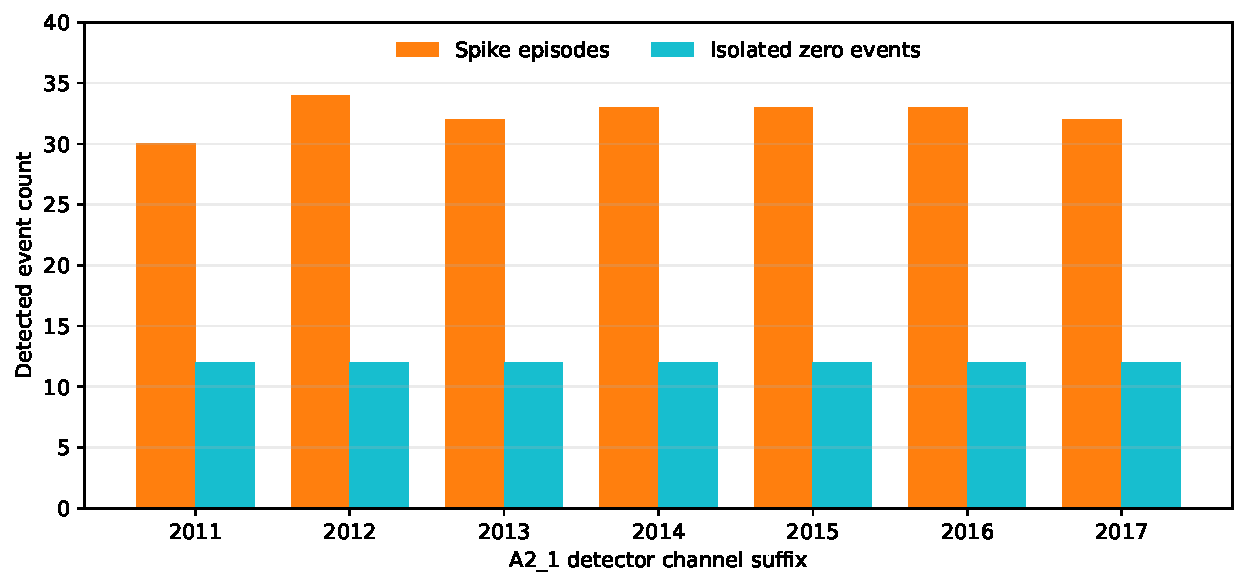
\includegraphics[width=0.88\textwidth]{fig07_a2_event_summary}
  \caption{代表性 A2 记录的确定性事件汇总（V2 占位图）。柱形表示各通道在固定规则下得到的短时偏离事件与孤立零值计数，并非已确认故障计数。正式版本将以局部多通道时序、记事板字段和紧凑摘要替换。}
  \label{fig:trace-placeholder}
\end{figure*}

基于上述摘要，本案例的检索意图是查找与测量完整性、同步事件、冗余或共享仪表上下文有关的可定位技术段落。该意图将观测限定为可核查的技术主题；第五章后续的扩库实验进一步表明，仅以语义近邻选择这些段落并不能保证预设核心资料仍在结果中可见。


\subsection{字符分块扩库协议：语义相似度与核心来源可见性可以背离}

\texttt{nomic-embed-text} 字符分块扩库协议显示，补充资料的加入不必降低最高余弦相似度，却可能迅速降低核心来源在前 10 个结果中的占比。每个非零扩库规模在每个分块配置下均基于 100 次补充资料随机抽样取平均，随后再聚合 17 个已保存配置；下列 $\pm$ 值表示配置间的标准差。中文测量短语 query 的 CorePriority@10 从仅含核心资料时的 1.00，在加入 5 份补充资料后降至 $0.10\pm0.09$，加入 10 份后降至 0；与此同时，平均最高余弦相似度由 0.55 上升至 0.63。英文 query 的下降较缓：加入 5 份补充资料后 CorePriority@10 为 $0.86\pm0.05$，在加入 45 份后为 $0.38\pm0.05$，最高余弦相似度则维持在约 0.69--0.70。

这一结果不表示补充资料不相关。相反，它表明当部署要求核心权威来源保持可见时，相关补充资料本身就足以改变无来源约束语义检索的结果构成。图~\ref{fig:scope-priority-placeholder} 同时呈现最高余弦相似度与 CorePriority@10 随扩库规模的轨迹，使读者直接看到“相似度提高或稳定”与“核心来源可见性下降”可以同时发生。

\begin{figure*}[t]
  \centering
  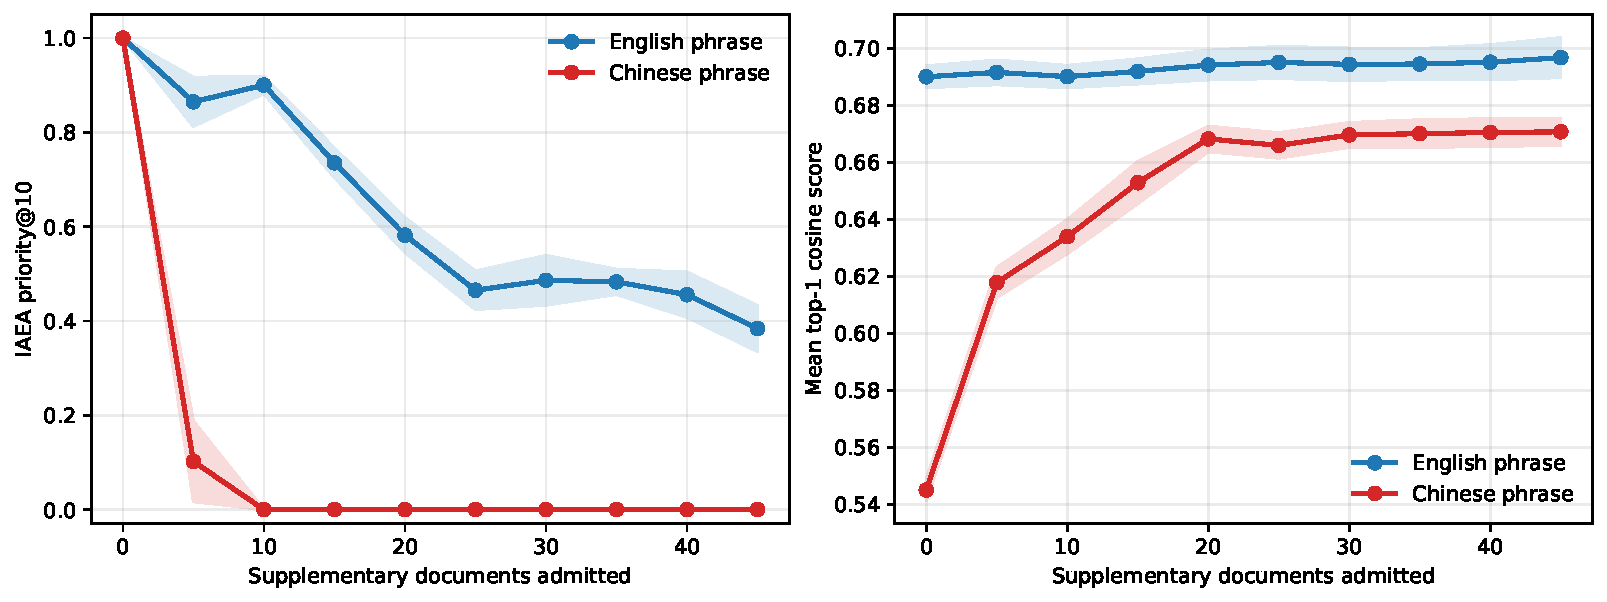
\includegraphics[width=0.94\textwidth]{fig08_scope_priority}
  \caption{资料扩展下的核心来源可见性与最高余弦相似度（V2 占位图）。结果聚合 17 个已保存分块配置；阴影表示配置间标准差。核心来源可见性可以下降，即使最高余弦相似度上升或保持稳定。正式版本将统一为 V3 的中文术语与版式。}
  \label{fig:scope-priority-placeholder}
\end{figure*}

\subsection{MiniLM encoder 对照：query、语言与分块的交互}

在保持资料库、top-10 规则和来源指标不变的 MiniLM 核查中，以两种 encoder 和三种字符分块设置比较简短基线 query 与由 observation packet 线索形成的技术细节 query。在加入 10 份补充资料时，技术细节 query 相对基线 query 的 CorePriority@10 变化在英文设置中介于 $-0.03$ 至 $+0.14$，在中文设置中介于 $-0.23$ 至 $+0.02$。因此，向 query 中加入观察细节并非总能提高核心来源可见性。

在两种 MiniLM encoder 分别配合三种字符分块设置所形成的六种配置上，平均结果也体现了这种不对称性：英文技术细节 query 的 CorePriority@10 为 0.65，高于英文基线 query 的 0.60；中文技术细节 query 为 0.52，低于中文基线 query 的 0.62。完整扩库轨迹进一步显示，各曲线均从 core-only 条件下的 1.00 出发，但其下降速度、交叉位置和对 query 细节的响应随语言与配置而变。图~\ref{fig:configuration-placeholder} 以 V2 的热图占位呈现这一交互；正式版本将压缩为与 V3 叙述一致的分面热图，不再在正文同时保留多张语言重复图、梯度图和轨迹图。

\begin{figure*}[t]
  \centering
  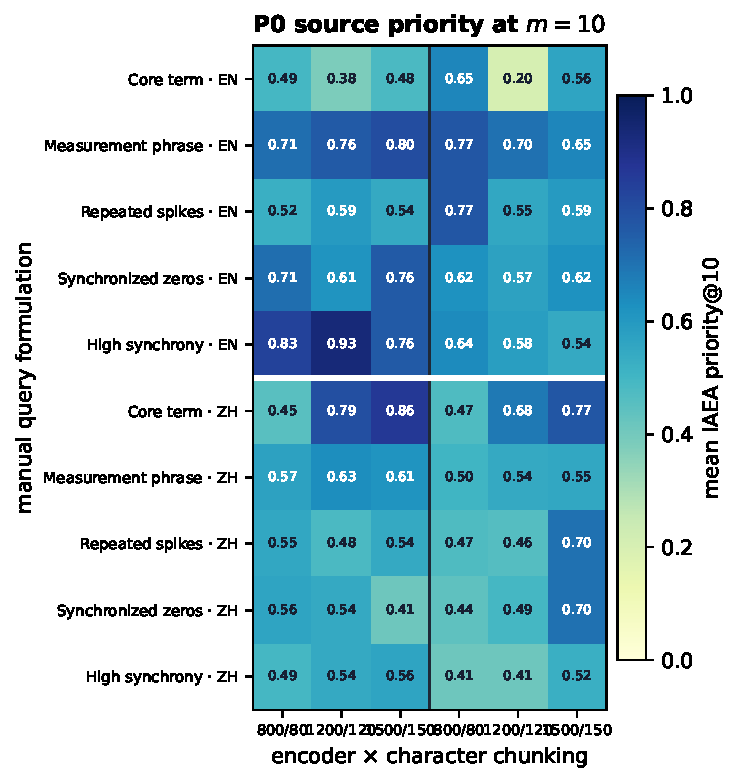
\includegraphics[width=0.54\textwidth]{fig13_p0_priority_heatmap}
  \caption{不同 query 与 encoder—分块配置下的核心来源可见性（V2 占位图，$m=10$）。该图显示 query 表述的作用随语言与配置而改变。正式版本将减少 query 行数，并以中文标签呈现。}
  \label{fig:configuration-placeholder}
\end{figure*}

配置交互并不意味着无法作出选择。在本资料库和来源要求下，已记录结果能够筛出来源可见性保持较好的候选组合。表 5.1 列出两类具有不同用途的例子：\texttt{nomic-embed-text} 的 800/120 字符分块配合英文核心术语 query，在加入 10 份补充资料时的 CorePriority@10 为 $0.92\pm0.12$，在全部 51 份补充资料加入后仍为 0.60；多语 MiniLM 的 800/80 设置配合“高度同步且无时间滞后”的英文观测 query，在相应条件下为 $0.83\pm0.18$ 和 0.40。前者更适合作为保持核心来源可见性的检索基线，后者则表明来自 observation packet 的具体线索也能形成具有较高来源可见性的案例检索表述。

\begin{table*}[t]
\centering
\footnotesize
\begin{tabular}{p{0.16\textwidth} p{0.16\textwidth} p{0.22\textwidth} p{0.16\textwidth} p{0.16\textwidth}}
\toprule
候选用途 & encoder 与分块 & query 表述 & CorePriority@10（$m=10$） & CorePriority@10（$m=51$） \\
\midrule
核心来源可见性基线 & \texttt{nomic-embed-text}，800/120 字符 & \texttt{neutron} & $0.92\pm0.12$ & 0.60 \\
同步通道现象的案例检索 & 多语 MiniLM，800/80 字符 & \texttt{neutron current measurement highly synchronized channels without time lag} & $0.83\pm0.18$ & 0.40 \\
\bottomrule
\end{tabular}
\end{table*}


这些候选组合不是跨语料库、任务或评价目标的“最优配置”。特别是，短核心术语 query 的来源可见性较高，并不自动表示其最贴合某一条具体记录；而 observation-derived query 更接近案例现象，也仍需检验所返回段落的实际相关性。表 5.1 的作用是为检索协议提供可复核的条件性选择依据：在以核心来源可见性为目标时，应优先从这类在扩库后仍保持较高 CorePriority@10 的组合中选择，再结合段落相关性和工程复核确定实际部署配置。

MiniLM encoder 对照与 \texttt{nomic-embed-text} 字符分块扩库协议共同表明：在本研究固定的资料库、检索规则和已测试 encoder 范围内，相关补充资料扩展后核心来源可见性下降的风险并非单一表示模型所致。由于两类协议的 query 集和部分分块设置不同，本文不直接比较其绝对余弦分数，也不据此排列 encoder 优劣；比较重点是各自协议内 CorePriority@10 随扩库规模的变化。技术细节 query 在不同语言和配置下的作用并不一致，因此结构化摘要应被理解为受控的检索表述，而非必然提高权威来源可见性的查询扩展。

\subsection{分块边界与检索单元核查}

固定词数分块的 MiniLM 对照表明，上述风险并非只出现在 \texttt{nomic-embed-text} 的字符分块中。多语种 MiniLM 对中文短语产生的最高余弦相似度约为 0.62--0.64，高于另一 MiniLM 的约 0.27；但随着补充资料加入，两种 encoder 的 CorePriority@10 均出现下降。语义表示对不同语言的近邻得分具有实质影响，却不能替代来源要求。

\texttt{nomic-embed-text} 索引上的 self-retrieval 则说明，检索单元的定义也会影响“找回”的含义。在一个 800/50 设置的 core-only 条件下，exact-chunk Recall@10 为 0.7625，而 same-document Recall@10 为 0.8625。该差异来自重叠分块：原始段落未必以同一 node 返回，但同一文档中的相邻段落可能已包含对应信息。因此，self-retrieval 结果用于解释 chunk 边界与段落定位，而不应与 CorePriority@10 混为同一种证据。

\begin{figure*}[t]
  \centering
  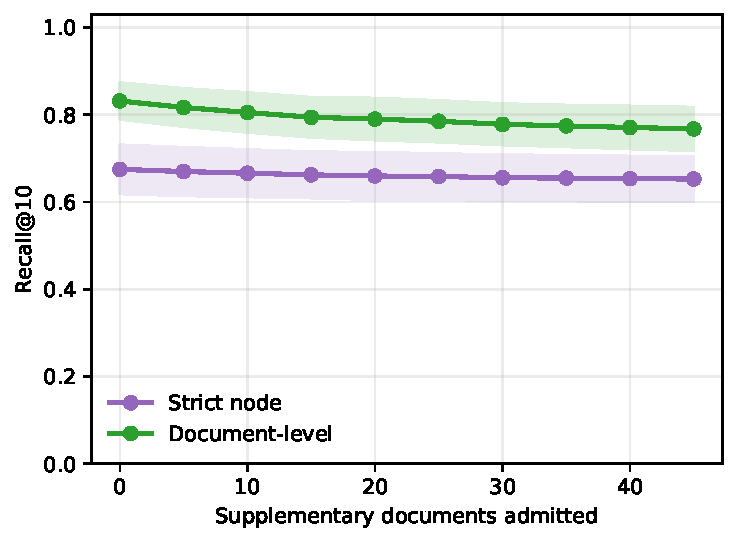
\includegraphics[width=0.84\textwidth]{fig17_self_retrieval_recall}
  \caption{self-retrieval 的 Recall@10 结果（V2 占位图）。该核查区分 exact-chunk 与 same-document 两种匹配标准，用于解释重叠分块下检索单元与段落定位的关系，而不衡量工程正确性。正式版本可与 MRR 合并重绘，或移至补充材料。}
  \label{fig:self-retrieval-placeholder}
\end{figure*}

\subsection{小结}

代表性 trace 说明，测量侧能够将无标签记录转换为可回指的检索线索；\texttt{nomic-embed-text} 字符分块扩库协议说明，证据侧若只依赖语义近邻，核心权威来源的可见性可能随相关资料的加入而丢失。MiniLM encoder 对照进一步表明：在本研究已测试的 encoder 范围内，这一风险并非单一向量表示所致；其幅度仍受 query、语言和分块方式共同影响，不能化约为某个组件的单一最优选择。与此同时，扩库后的来源可见性指标能够筛出条件性候选配置，为检索协议选择提供实证依据。由此，来源 metadata 与显式来源策略不是检索实现的附属信息，而是 measurement-to-evidence interface 中需要被设计和评价的部分。

\section{结论}

本文面向缺乏统一样本级故障真值的多通道中子电流历史档案，将研究目标从自动故障分类转为可追溯的诊断辅助：先将原始测量转化为工程师可复核的观察，再使后续技术解释能够回指至适当的资料依据。为此，本文构建了 measurement-to-evidence interface。测量侧以确定性脚本生成并保存 observation packet；紧凑摘要直接由稳定的结构化字段形成，作为证据侧的受控检索意图；语言模型只组织已获得的观察、资料段落和候选解释，不从原始波形自行生成测量事实，也不确认物理机理。

代表性 trace 表明，这一接口能够把长时、多通道记录压缩为可检查的观察链。A2 记录中的孤立零值、短时偏离、通道间时间关系和极值位置均可回指到相应的输入、参数与工具输出。跨通道重复的零值时间因而可被保留为测量完整性或共享仪表上下文的检索线索，而不会被直接提升为某一种已确认故障。该结果说明，在没有统一标签的条件下，观测的可回指性本身构成了后续工程复核的必要基础。

证据侧实验表明，语义相似度不能单独承担来源治理的角色。在 \texttt{nomic-embed-text} 字符分块扩库协议中，相关补充资料加入后，最高余弦相似度可以提高或保持稳定，而前 10 个结果中核心权威资料的占比却会下降。MiniLM encoder 对照中同样观察到这一风险，说明该现象不宜归因于单一向量表示模型。资料范围、query 表述、语言、encoder 和分块方式共同改变检索结果；尤其是，技术细节 query 并不必然提高前 10 个结果中核心资料的占比。与此同时，实验能够按扩库后的 CorePriority@10 筛出这一占比保持较高的候选组合，为检索协议的条件性选择提供依据。由此，补充资料不应被视为无关噪声，但若应用要求特定权威资料集合保持在检索结果前列，来源 metadata 与来源策略必须被明确纳入检索设计和评价。

检索单元的核查还表明，重叠分块下“找回同一段落”与“找回同一文档”回答不同问题。同文档检索表现高于严格同分块检索，说明相邻分块可能保留了所需内容；因此，分块边界、段落定位与来源可见性需要分别报告，而不能以单一检索分数替代。综合这些结果，本文的结论是：无标签工程时序的安全使用依赖于“先描述、后判断”的责任分工——确定性工具产生可回指观察，检索系统定位带来源信息的技术证据，语言模型组织受证据约束的候选解释，工程师保留机理判断和最终决策。后续若能接入脱敏的运行/维护背景并获得领域专家复核，可在该接口之上进一步检验机理假设、段落支持与工程有用性。


\bibliographystyle{elsarticle-num}
\bibliography{refs}
\end{document}
